\chapter{Discussion}
\label{cha:discussion}

\section{Results}
\label{sec:discussion-results}

After analysing the results from the imputation experiments and the prediction generalisation, the structural time series and multivariate Prophet model have been chosen for each stage, respectively. Figure \ref{fig:final_pipeline} shows how the pipeline has been defined. 

\begin{figure}[H]
\centering
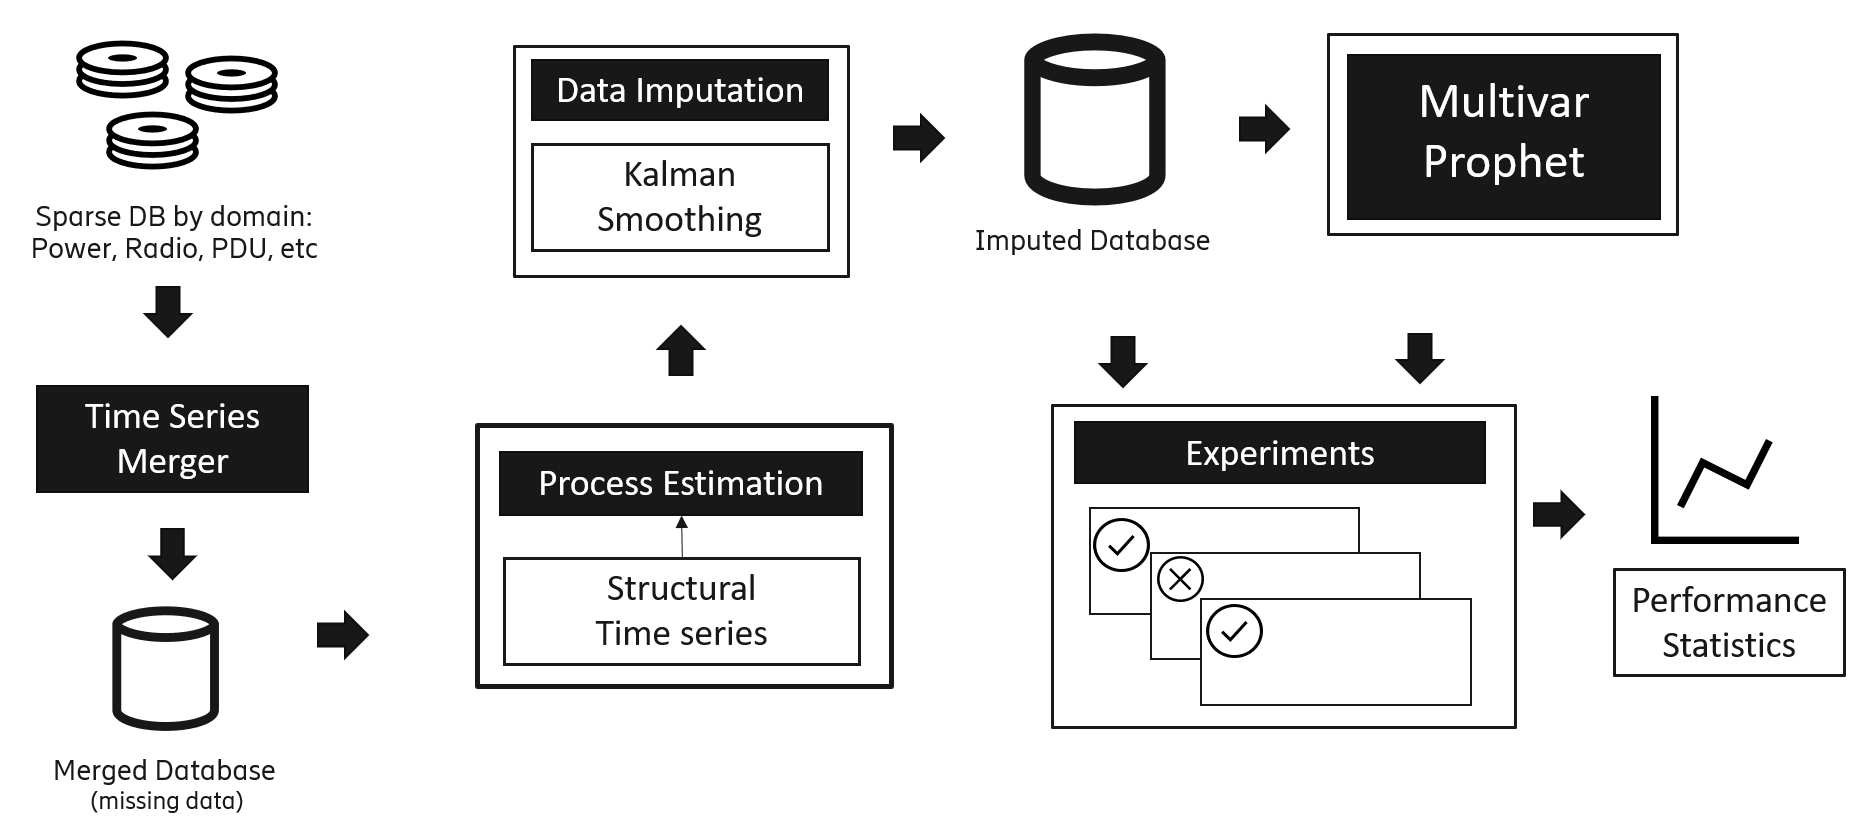
\includegraphics[width=1\linewidth]{pipeline_final}
\caption{Final pipeline architecture}
\label{fig:final_pipeline}
\end{figure}


In the imputation stage, the Auto-ARIMA model has shown to be unstable for some features in the dataset, whereas the structural models have not. This inconsistency should not be understood as a failure of the SARIMA approach itself but as an instability in the auto-ARIMA algorithm not reaching a proper model through its heuristics. Thus, even though the auto-ARIMA algorithm has been published and implemented in a popular library, it still has some arbitrary steps.

When it comes to comparing the baselines performances against the univariate Prophet model, it can be seen that the latter sometimes performs even worse than the baselines, which might induce some critical thoughts about the Prophet model as an insufficient framework. Nonetheless, when adding exogenous regressors, the model shows its potential by lowering the error rates significantly, reaching $R^2>0.8$ values, which can be considered a reasonable approximation due to the nature of the target signal.

Although a power headroom derivation from the \ac{psu} utilisation has been presented, the $n$-level criteria have not been tested in a case that meets them and triggers an alarm.


\section{Methods}
\label{sec:discussion-methods}

\subsection{Time series merging}

In the current case, to build the database, it has been decided to merge the time series with an outer join and then impute the missing data rather than using inner joins and reduced data. Nevertheless, this does not mean that this approach is always the recommended approach. A further study that could have been done is to extract the \emph{longest} uncorrupted piece of time series $\{\bm{U}_t\} \subseteq \{\bm{Y}_t\}$ and run statistical tests to measure their similarities and determine if subseries $\{\bm{U}_t\}$ is \emph{representative} of the complete series $\{\bm{Y}_t\}$. 

This scenario could happen when having a very long time series of highly seasonal data. Unfortunately, it has not been the case for the available data since extrapolating two months to an entire year can be considered already only a proof of concept. Trimming the time series, even more is undesired.


\subsection{Time series imputation}
\label{subsec:discussion-methods-imputation}

Only univariate approaches have been used to estimate the model and smoothen the signals, which implicitly --and naively-- implies that the features are independent and no correlations can be found between them. This decision was intentionally made to set a baseline and, as the first attempt on this domain within the company, prioritising simplicity over sophistication.

It should be noted that multivariate imputing techniques could improve the processing time and the imputation accuracy.

\subsection{Forecast}

The Prophet model was chosen as a predictive model for its novelty, flexibility, well-proven usage in the social networks industry, and good performance in the long-range forecasts. Besides its theoretical attractiveness, it is also well suited for time-limited work due to its well-designed \acp{api} and available documentation. Nonetheless, there are no strong arguments to state that it is the \emph{best-suited} model since it has been only compared against the baselines. 

The baselines have been implemented using only univariate approaches. Therefore comparing the multivariate Prophet model against them might not be the fairest. Other multivariate methods might be used as baselines in such case.  

Other than the Prophet model, a boosted decision trees regressor was explored using XGBoost, which showed promising results. Nonetheless, its current implementation status can be considered half-done and, therefore, its results cannot be conclusive.


\section{Ethical considerations}
\label{sec:work-wider-context}

The project aims to open a research line towards decreasing of \acp{mno} operational costs. Nonetheless, this is not limited to a purely economic benefit to the companies. Maintenance duties can imply some risks to the field workforce when, for instance, the \ac{rbs} is located in a remote location. Therefore, this project effects will be also beneficial for the field personnel. 

Environmentally wise, reducing the number of trips and interventions in remote locations, which could be close to nature wildlife, will also reduce the pollution levels related to them and wildlife invasions.

Although the project's domain is in mobile communication, it is directly related to human behaviours. Therefore, analysing how this may be affected by social biases and whether its effects could be more beneficial towards one group of people or detrimental to others is, in fact, a moral obligation from the researcher's and developer's perspective. 

In that line, it is crucial to state that different groups of people behave differently. Therefore, the seasonalities learnt from data from one country may not reflect the customs in others, especially when it is related to holidays or temperature. As a consequence, it can be stated that when a system of this nature is deployed as a service, it needs to learn from data coming from the region where it is being deployed or some other statistically similar data. 